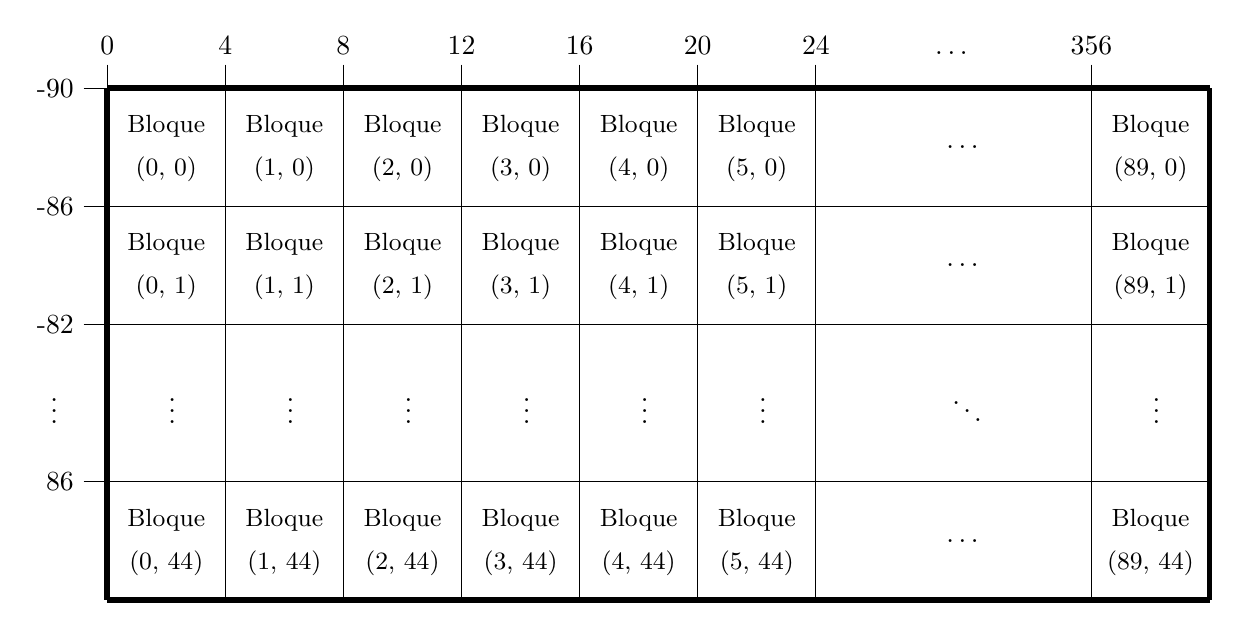
\begin{tikzpicture}
    \draw[line width=2pt] (0,0) -- (14,0);
    \draw[line width=2pt] (0,-6.5) -- (14,-6.5);
    \draw[line width=2pt] (0,0) -- (0,-6.5);
    \draw[line width=2pt] (14,0) -- (14,-6.5);

    % Labels
    \foreach \i in {0, 1.5, 3,...,10}
    {
        \draw (\i,0.3) -- (\i,-6.5);
        \pgfmathtruncatemacro{\label}{4*\i/1.5};
        \node[anchor=south] at (\i, 0.3) {\label \si{\degree}};
    }
    \draw (12.5,0.3) -- (12.5,-6.5);
    \node[anchor=south] at (12.5, 0.3) {356\si{\degree}};
    \node[anchor=south] at (10.75, 0.3) {\ldots};

    \foreach \i in {0, -1.5, -3}
    {
        \draw (-0.3, \i) -- (14, \i);
        \pgfmathtruncatemacro{\label}{90+4*\i/1.5};
        \node[anchor=east] at (-0.3, \i) {-\label \si{\degree}};
    }

    \draw (-0.3, -5) -- (14, -5);
    \node[anchor=east] at (-0.5, -4) {\vdots};
    \node[anchor=east] at (-0.3, -5) {86\si{\degree}};

    %Blocks
    \foreach \i in {1.5, 3, ...,10}
    {
        \pgfmathtruncatemacro{\bloquei}{\i/1.5 - 1};
        \foreach \j in {-1.5, -3}{
            \pgfmathtruncatemacro{\bloquej}{-\j/1.5-1};
            \node[anchor=south] at (\i-0.75, \j+0.75) {\small{Bloque}};
            \node[anchor=north] at (\i-0.75, \j+0.75) {\small{(\bloquei, \bloquej)}};

        }
        % \draw (\i,0.3) -- (\i,-6.5);
        % \pgfmathtruncatemacro{\label}{4*\i/1.5};
        
    }

    % Bloques extremo izquerda
    \node[anchor=south] at (13.25, -0.75) {\small{Bloque}};
    \node[anchor=north] at (13.25, -0.75) {\small{(89, 0)}};

    \node[anchor=south] at (13.25, -2.25) {\small{Bloque}};
    \node[anchor=north] at (13.25, -2.25) {\small{(89, 1)}};

    \node[anchor=south] at (13.25, -5.75) {\small{Bloque}};
    \node[anchor=north] at (13.25, -5.75) {\small{(89, 44)}};

    % Bloques abajo
    \foreach \i in {1.5, 3, ...,10}
    {
        \pgfmathtruncatemacro{\bloquei}{\i/1.5 - 1};
        \node[anchor=south] at (\i-0.75, -5.75) {\small{Bloque}};
        \node[anchor=north] at (\i-0.75, -5.75) {\small{(\bloquei, 44)}};
    }


    %Puntitos
    \foreach \i in {1.5, 3, ..., 10, 14}
    {
        \node[anchor=east] at (\i-0.5, -4) {\vdots};
    }

    \foreach \j in {0, -1.5, -5}
    {
        \node[anchor=east] at (11.25, \j-0.75) {\ldots};
    }

    \node[anchor=east] at (11.25, -4) {$\ddots$};


\end{tikzpicture}